\documentclass{esannV2}
\usepackage{graphicx}
\usepackage[utf8]{inputenc}
\usepackage{amssymb,amsmath,array}

\usepackage{hyperref}
\usepackage{listings}
\lstset{
  language=bash,
  basicstyle=\ttfamily
}
%***********************************************************************
% !!!! IMPORTANT NOTICE ON TEXT MARGINS !!!!!
%***********************************************************************
%
% Please avoid using DVI2PDF or PS2PDF converters: some undesired
% shifting/scaling may occur when using these programs
% It is strongly recommended to use the DVIPS converters, and to submit
% PS file. You may submit a PDF file if and only if you use ADOBE ACROBAT
% to convert your PS file to PDF.
%
% Check that you have set the paper size to A4 (and NOT to letter) in your
% dvi2ps converter, in Adobe Acrobat if you use it, and in any printer driver
% that you could use.  You also have to disable the 'scale to fit paper' option
% of your printer driver.
%
% In any case, please check carefully that the final size of the top and
% bottom margins is 5.2 cm and of the left and right margins is 4.4 cm.
% It is your responsibility to verify this important requirement.  If these margin requirements and not fulfilled at the end of your file generation process, please use the following commands to correct them.  Otherwise, please do not modify these commands.
%
\voffset 0 cm \hoffset 0 cm \addtolength{\textwidth}{0cm}
\addtolength{\textheight}{0cm}\addtolength{\leftmargin}{0cm}

%***********************************************************************
% !!!! USE OF THE esannV2 LaTeX STYLE FILE !!!!!
%***********************************************************************
%
% Some commands are inserted in the following .tex example file.  Therefore to
% set up your ESANN submission, please use this file and modify it to insert
% your text, rather than staring from a blank .tex file.  In this way, you will
% have the commands inserted in the right place.

\begin{document}
%style file for ESANN manuscripts
\title{NARIZ ARTIFICIAL: SENSORES DE GAS PARA MONITORIZACIÓN DE ACTIVIDAD DOMÉSTICA}

%***********************************************************************
% AUTHORS INFORMATION AREA
%***********************************************************************
\author{Jorge Durán León, Jaime Enríquez Ballesteros, Marcos de las Heras Roncero
%
% Optional short acknowledgment: remove next line if non-needed
%\thanks{This is an optional funding source acknowledgement.}
%
% DO NOT MODIFY THE FOLLOWING '\vspace' ARGUMENT
\vspace{.3cm}\\
%
% Addresses and institutions (remove "1- " in case of a single institution)
  Escuela Politécnica Superior, Fundamentos de Aprendizaje Automático \\
%Address of First Author's school - Country of First Author's
%school
%
% Remove the next three lines in case of a single institution
%\vspace{.1cm}\\
%2- School of Second Author - Dept of Second Author \\
%Address of Second Author's school - Country of Second Author's school\\
}
%***********************************************************************
% END OF AUTHORS INFORMATION AREA
%***********************************************************************

\maketitle

\begin{abstract}
Resumen del trabajo realizado en 100 palabras.
\end{abstract}

\section{Introducción}

El proyecto que se ha realizado trata sobre el análisis de un conjunto de datos recogidos por 8 sensores de gas, un sensor de temperatura y un sensor de humedad. Estos sensores fueron expuestos a estímulos por la presencia de vino y plátanos. Además, se recogen datos de la respuesta a la no presencia de ninguno de ellos. El objetivo del proyecto es la clasificación de las respuestas de los sensores a los estímulos previamente dichos. Para ello primero se analizarán los datos del dataset mediante técnicas de preprocesamiento para ver que pueden ofrecer esos datos a la hora de clasificar las respuestas. Después, se elegirán los modelos de aprendizaje automático supervisado que mejor nos convengan para dicho dataset. Por último, se compararán los resultados de los distintos modelos y razonaremos si son resultados aceptables y qué modelos han dado mejores resultados.

\section{Descripción del Dataset}
El dataset proporcionado de los datos de los sensores está compuesto por dos archivos: el archivo HT\_Sensor\_dataset.dat; que contiene el identificador de la inducción, instantes de tiempo para cada inducción y los datos de los sensores para cada inducción en esos instantes de tiempo, y el archivo HT\_Sensor\_metadata.dat; que contiene para cada inducción su identificador, el día en que fue realizada, el estímulo usado para la inducción, y el intervalo de tiempo de la inducción, que está dividido en tiempo inicial y duración de la misma. \\
En este último dataset hay 3 clases distintas para clasificar, que se corresponden con los estímulos que reciben los sensores:  vino (wine), plátano (banana) y ningún estímulo (background). En total se realizan 100 inducciones, donde  36 se realizan con vino, 33 con plátano y 31 son background. De esas 100 inducciones se recogen 928991 datos en distintos instantes de tiempo. Al analizar los datos se puede comprobar que no hay datos para la inducción con el identificador 95, por lo que esta instancia es descartada del análisis. Además de los datos recogidos durante la inducción, se nos ofrecen los datos de los instantes previos y posteriores de la inducción. Esta división del tiempo se puede calcular fácilmente para cada inducción con la ayuda de los datos del tiempo del archivo de los metadatos (HT\_Sensor\_metadata.dat), por lo que podemos distinguir para cada experimento estos tres periodos diferenciados. Comprobamos que para los experimentos con identificadores 14 y 76 no tenemos datos posteriores a la inducción, por lo que también los descartamos, quedando 97 instancias válidas. \\
Los atributos del dataset son numéricos y reales, por lo que se pueden utilizar las medidas características de la distribución de cada atributo para analizarlo. Estas medidas pueden ser de centralización, como la media, o de dispersión, como la varianza. Con estas medidas se puede ver como se comporta cada sensor frente a los estímulos. En el siguiente apartado se verá un pequeño resumen sobre el  análisis llevado a cabo sobre los datos y el proceso a seguir para obtener los atributos que serán utilizados para entrenar a los modelos en el apartado 4.

\section{Análisis  de los Datos y Elección de Atributos}
La mayoría de funciones utilizadas para el análisis de los datos y el preprocesamiento previo al entrenamiento de modelos se pueden encontrar en el fichero \textit{Preprocess.py}. La única excepción es la función utilizada para la representación de instancias a lo largo del tiempo que encontramos en el fichero \\ \textit{Plot\_Induction\_Figure.py} que se facilita en [1]. Todas las operaciones de este apartado (así como del resto) pueden encontrarse en \textit{proyecto.ipynb}. Se utilizan los módulos de Pandas [2], NumPy [3], Sci-kit Learn [4] y Matplotlib [5]. \\
El primer paso para el análisis será representar los experimentos para cada clase y fijarse en qué atributos pueden marcar la diferencia a la hora de clasificar. La Figura~\ref{fig:banvswinvsbck} muestra al progresión de los sensores para 3 experimentos (id=0, id=1, id=69), uno por clase. \\

\begin{figure}[b!]
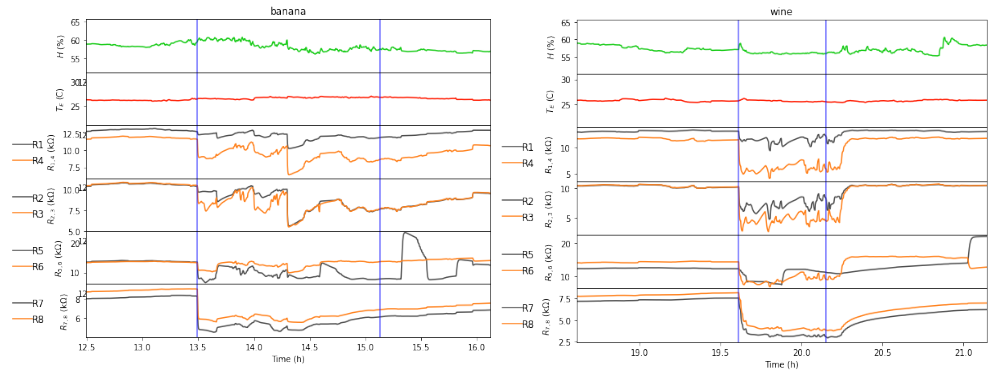
\includegraphics[scale=0.35]{img/banvswin.png}
\centering
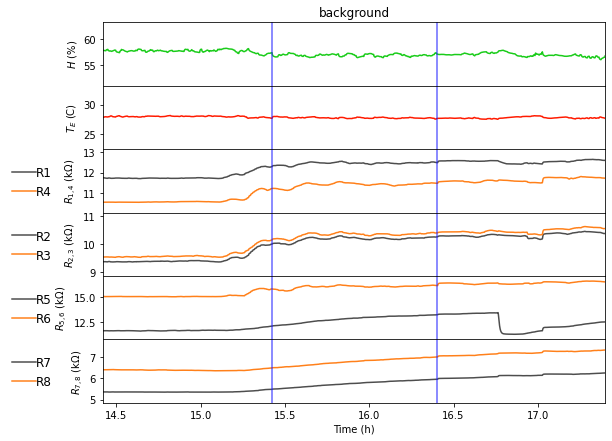
\includegraphics[scale=0.3]{img/background_69.png}
\caption{Comparación entre clases}\label{fig:banvswinvsbck}
\end{figure}


Se puede observar como los atributos de temperatura y humedad obtienen valores  y varianzas muy similares independientemente de la clase. Al representar esta relación, se comprueba como estos atributos no nos van a ayudar a predecir la clase de cada experimento, al no estar correlacionados. Por otro lado, se observa como cuando la humedad es más alta, los sensores obtienen unos resultados más fluctuantes que con humedad baja. Se puede ver claramente cuando se representan los experimentos con id=0 e id=10 (se muestra en el código). Se estima que los atributos de temperatura y humedad pueden ser útiles si se utilizan junto a otros atributos para la clasificación, pero no si se utilizan solos. \\

Por otro lado, los sensores obtienen estimulaciones muy diferentes entre ellos según la clase. La fluctuación de los sensores durante la estimulación del experimento (entre las dos líneas azules)  es muy pronunciada para el vino, seguido del plátano y muy poco notable cuando no se introduce ningún elemento en el sensor. En la Figura~\ref{fig:banvswinvsbck} se muestra muy claramente. Por lo tanto, la varianza de cada sensor puede ser un posible atributo para nuestro modelo. \\

Además, como se muestra en el notebook, la media y mediana de los sensores son muy similares independientemente de la clase que utilicemos. No serán considerados como atributos útiles para el modelo final. Lo mismo sucede con los valores máximos y mínimos de cada sensor. Aunque los valores varían mucho dependiendo de cada ejemplo, no existe un patrón que se repita según la clase. En el caso de utilizar alguna de estas cuantías como atributo de un modelo, se obtienen resultados muy malos. Modificando mínimamente el código se puede comprobar este suceso. \\

Volviendo a la variabilidad de los sensores, la distancia entre el máximo y mínimo valor de cada sensor (que será referido como amplitud) también podría ser útil a la hora de clasificar. Como con la varianza, se obtienen unos valores mayores para los casos en los que el objeto es vino en comparación con un plátano o cuando no se inserta nada.  Se puede considerar por lo tanto, que los atributos que se tomarán para entrenar a nuestro modelo se basarán en la variabilidad de cada uno de los sensores, al ser las cuantías que más correlación observada obtienen con la correspondiente clase. Tras calcular  la varianza y amplitud de cada sensor, se obtienen 16 atributos para cada ejemplo. A estos atributos se les añaden las medias de la humedad y temperatura, que como se explica anteriormente, pueden ayudar en el proceso de clasificiación, aunque por sí solos no sean útiles. En total se tendrán 18 atributos de entrada por ejemplo del dataset.\\

Todos los atributos serán normalizados previo al entrenamiento del modelo. Este paso mejora la predicción de los modelos al no utilizar distintas escalas para cada atributo . Para este proyecto se utiliza el método de Sci-kit Learn  \textit{StandardScaler} que normaliza los atributos restando su correspondiente media y dividiendo el resultado por la desviación estándar. Tras esta transformación se puede comenzar a entrenar a los modelos. En el siguiente apartado se describe el proceso seguido.

\section{Modelos Propuestos}

A la hora de definir los distintos conjuntos de datos de entrenamiento y prueba, se deberá prestar atención a mantener la misma proporción de cada clase en cada conjunto. De este modo no habrá infrajuste sobre una clase que tenga poca presencia en el conjunto de entrenamiento. Para ello se hace uso del método de Sci-kit Learn \textit{StratifiedShuffleSplit} que mezclará el conjunto de datos entero y dividirlo entre conjunto de entrenamiento y prueba. Se utilizará un conjunto de prueba del 10\% de tamaño del conjunto total.\\

Utilizando el módulo de  Python \textit{LazyPredict} se podrá hacer una rápida evaluación sobre qué modelos obtendrán buenos resultados. Uno de los modelos del módulo puede entrenar muchos algoritmos de clasificación de Sci-kit Learn[4], xgboost [8] o lightgbm [9] a partir de unos parámetros de entrada y calcular el error de predicción sobre un conjunto de prueba calculando "F-1 Score" o "Accuracy" para cada modelo. 
Debido a que este conjunto de datos es tan pequeño y es probable que los modelos se sobreajusten sobre los datos de entrenamiento, causando que las predicciones sean muy erróneas, el proceso de entrenamiento y validación de   \textit{LazyPredict}  se repetirá un total de 30 veces. De este modo se dividirá el conjunto de datos cada una de las veces de manera distinta, se almacenarán los resultados y se calculará la media para obtener así el mejor modelo sobre las 30 iteraciones. \\ 

Se decide probar a utilizar un modelo de redes neuronales y comprobar su eficiencia sobre nuestro conjunto de datos. Se implementa mediante el módulo de Python, Keras [7]. Se utilizará una red neuronal de una capa oculta con la arquitectura que muestra la Figura ~\ref{fig:nn}, con un input de 18 atributos, una capa oculta de 10 perceptrones y un output de 3 probabilidades. Las dos primeras capas con una función de activación ReLu y la última Softmax, para calcular las probabilidades de cada ejemplo. \\


Se decide probar a utilizar un modelo de redes neuronales y comprobar su eficiencia sobre nuestro conjunto de datos. Se implementa mediante el módulo de Python, Keras [7]. Se utilizará una red neuronal de una capa oculta con la arquitectura que muestra. \\ 

Otro modelo a considerar es \textit{OneVsRest} para predecir los casos de una sola clase. Para ello, se emplean las varianzas de los valores de los 8 sensores y los separamos en antes durante y después. 
Con el objetivo de seleccionar el mejor clasificador posible para cada caso, se comprobará de forma empírica que combinación de variaciones es la mejor para la predicción de cada clase. Para la clasificación se empleará el algoritmo de clasificación \textit{RandomForestClassifier}. \\



\section{Discusión de Resultados}
Sobre los 28 modelos, los mejores cinco que se obtienen (y su correspondientes métricas) se muestran el la Tabla~\ref{tab:lazypred}. Los resultados pueden variar según la ejecución pero estos modelos siempre se encuentran entre los cinco primeros.\\

\begin{table}[!]
  \centering
  \begin{tabular}{|c|c|c|}
    \hline
    Modelo & Accuracy & F1-Score \\
    \hline
    RandomForestClassifier & 0.76 & 0.75 \\ 
	ExtraTreesClassifier & 0.74 & 0.74 \\ 
	XGBClassifier & 0.74 & 0.73 \\ 
	LogisticRegression & 0.74 & 0.72 \\ 
	LinearSVC & 0.73 & 0.71 \\ 
    \hline
  \end{tabular}
  \caption{Precisión de los distintos modelos}\label{tab:lazypred}
\end{table}

%Los resultados podrán variar según la ejecución pero entre los cinco mejores, siempre se repiten los mostrados en la Tabla~\ref{tab:lazypred}.\\

A partir de estos resultados, se deciden utilizar  los cinco modelos: \textit{LogisticRegression, KNeighborsClassifier, RandomForestClassifier,LinearSVC y XGBClassifier}. Utilizando la última división del conjunto de datos de las 30 iteraciones, se realiza una validación cruzada para cada modelo con nuestros datos de entrenamiento con el número de folds siendo igual a 10. De este modo, se realizarán más validaciones y los modelos podrán ser entrenados sobre la mayoría de datos del conjunto de entrenamiento. A partir de las valdaciones cruzadas podremos obtener una matriz de confusión. Esto es posible gracias al método de Sci-kit Learn  textit{cross\_val\_predict} que almacena todas las predicciones sobre cada fold de la validación cruzada.  Los resultados se muestran en la Figura ~\ref{fig:cm}.  \\

\begin{figure}[b!]
\centering
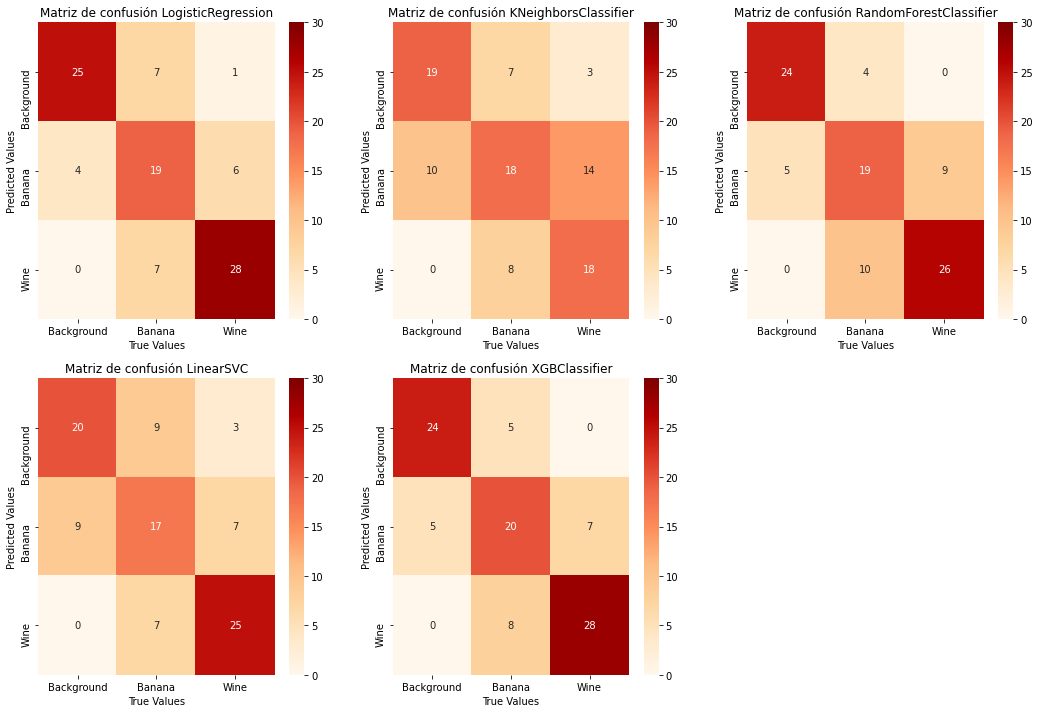
\includegraphics[scale=0.3]{img/matrices_confusion.png}
\caption{Matrices de confusión sobre distintos modelos}\label{fig:cm}
\end{figure}




%Los malos resultados de la red neuronal motivan a utilizar uno de los modelos anteriores de Sci-kit Learn. 
Observando las matrices de confusión, se eligen los modelos de Regresión Logística (LogisticRegression) y de "Extreme Gradient Boosting"[8]  (XDBClassifier), al ser los que mejor exactitud ("accuracy") obtienen. Estos dos modelos serán refinados mediante el módulo de Sci-kit Learn, \textit{GridSearchCV} para obtener los valores de sus parámetros  que maximicen el acierto en las predicciones. \\
Con los modelos obtenidos tras el refinamiento de parámetros se realiza un entrenamiento y una predicción sobre los conjuntos de entrenamiento y de prueba, correspondientemente. Para el modelo de "Extreme Gradient Boosting" se obtiene un acierto del 80\% mientras que para el de regresión logística un acierto del 70\%. Como se menciona anteriormente, estos valores pueden variar según se ejecute otra vez, pero los resultados no deberían de cambiar más del 5\%. \\

Podemos ver el resultado de la clasificación mediante redes neuronales en la Figura ~\ref{fig:nn}, con un input de 18 atributos, una capa oculta de 10 perceptrones y un output de 3 probabilidades. Las dos primeras capas con una función de activación ReLu y la última Softmax, para calcular las probabilidades de cada ejemplo. La Figura ~\ref{fig:nn} también muestra los malos resultados de validación del modelo, con un 50\% de accuracy y un error que baja muy ligeramente a medida que aumentan las épocas.   \\

\begin{figure}[b!]
\centering
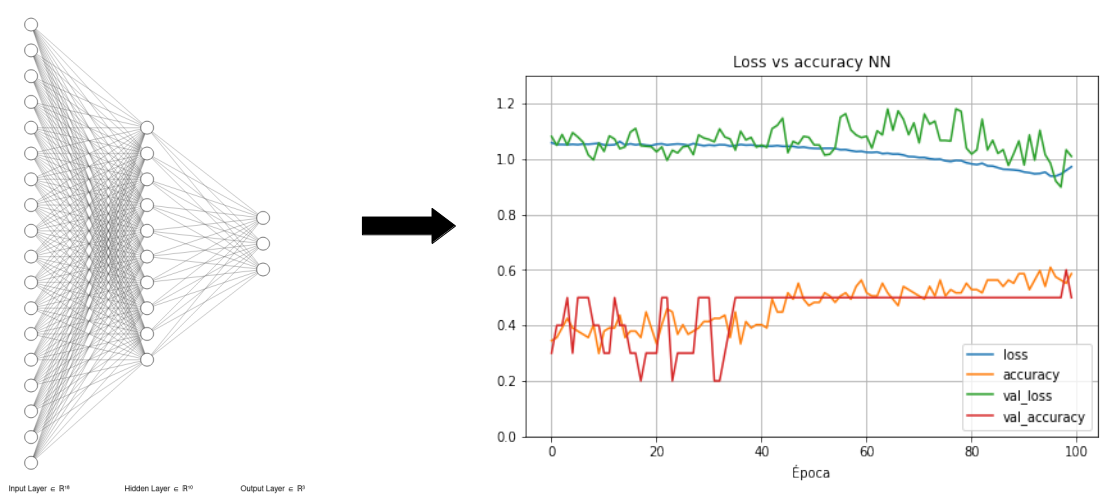
\includegraphics[scale=0.3]{img/nn.png}
\caption{Matrices de confusión sobre distintos modelos}\label{fig:nn}
\end{figure}

Para los clasificadores \textit{OneVsRest} se ha comprobado de forma empírica que las mejores combinaciones de varianzas son:
\begin{itemize}
  \item varianzas durante la inducción para los casos de tipo banana.
  \item varianzas durante y después de la inducción para los casos de tipo wine.
  \item varianzas antes, durante y después de la inducción para los casos de tipo background.
\end{itemize}


\begin{table}[!]
  \centering
  \begin{tabular}{|c|c|c|}
    \hline
    Modelo & Accuracy & F1-Score \\
    \hline
    Banana & 0.75 & 0.64 \\ 
	Wine & 0.9 & 0.9 \\ 
	Background & 0.95 & 0.915 \\ 
    \hline
  \end{tabular}
  \caption{Precisión por clase}\label{tab:lazypred}
\end{table}

Mediante los resultados presentes en la Tabla~\ref{tab:lazypred} se obtienen valores aceptables para la predicción de la clase banana y muy acertados para las otras dos clases. Estas afirmaciones quedan respaldadas por los curvas ROC presentes en la la figura ~\ref{fig:roc}, donde podemos ver que en el caso de banana, la tasa de acierto sube mediante escalones con un crecimiento reducido, mientras que en el caso de wine sigue una forma logarítmica, y en el caso background toma practicamente el valor de 1 en el momento inicial. \\

\begin{figure}[b!]
\centering
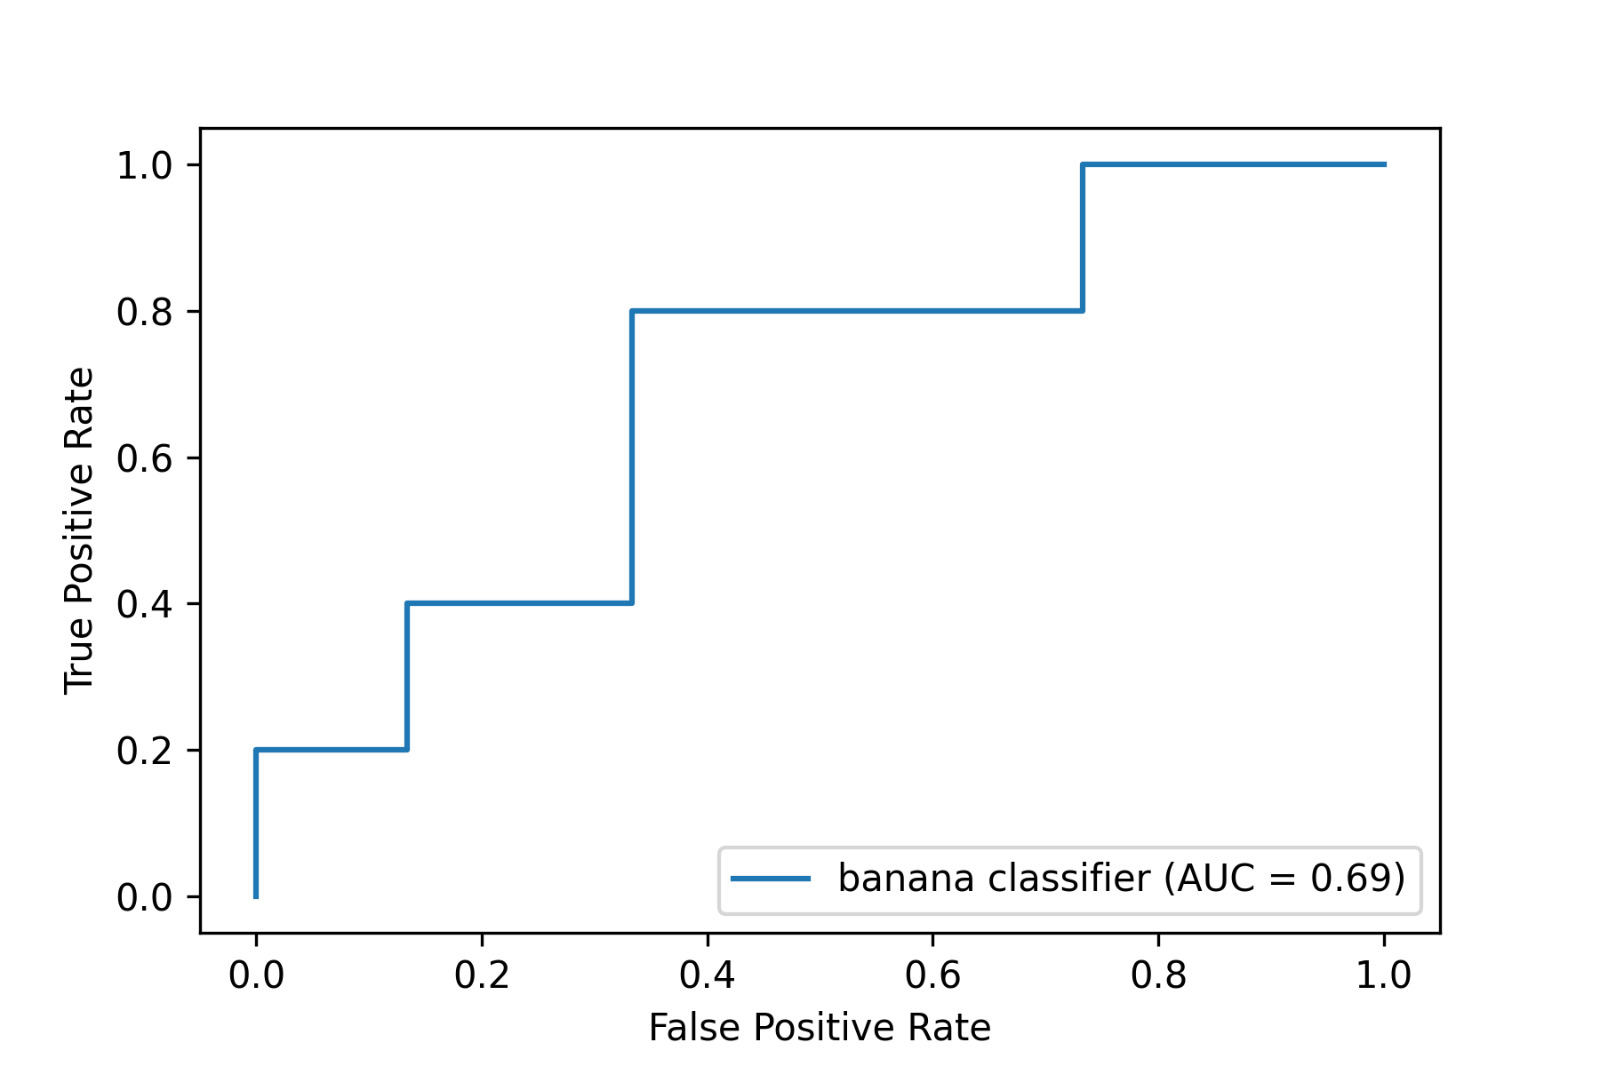
\includegraphics[scale=0.3]{img/banana.png}
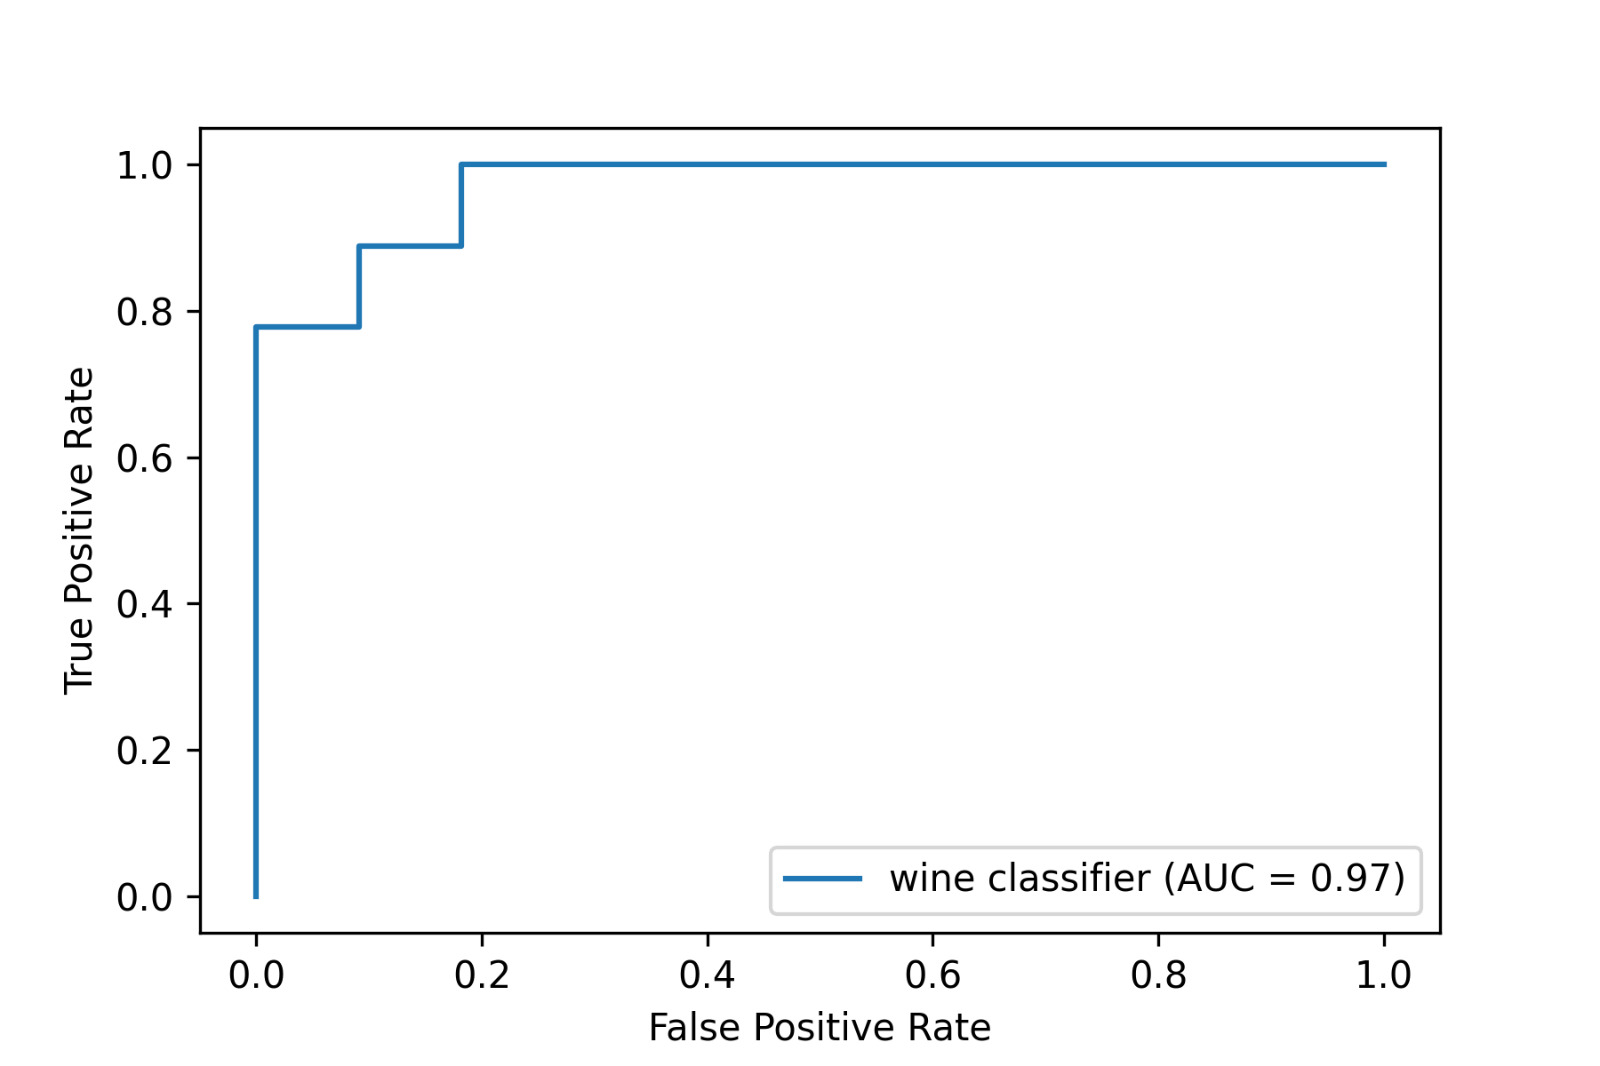
\includegraphics[scale=0.3]{img/wine.png}
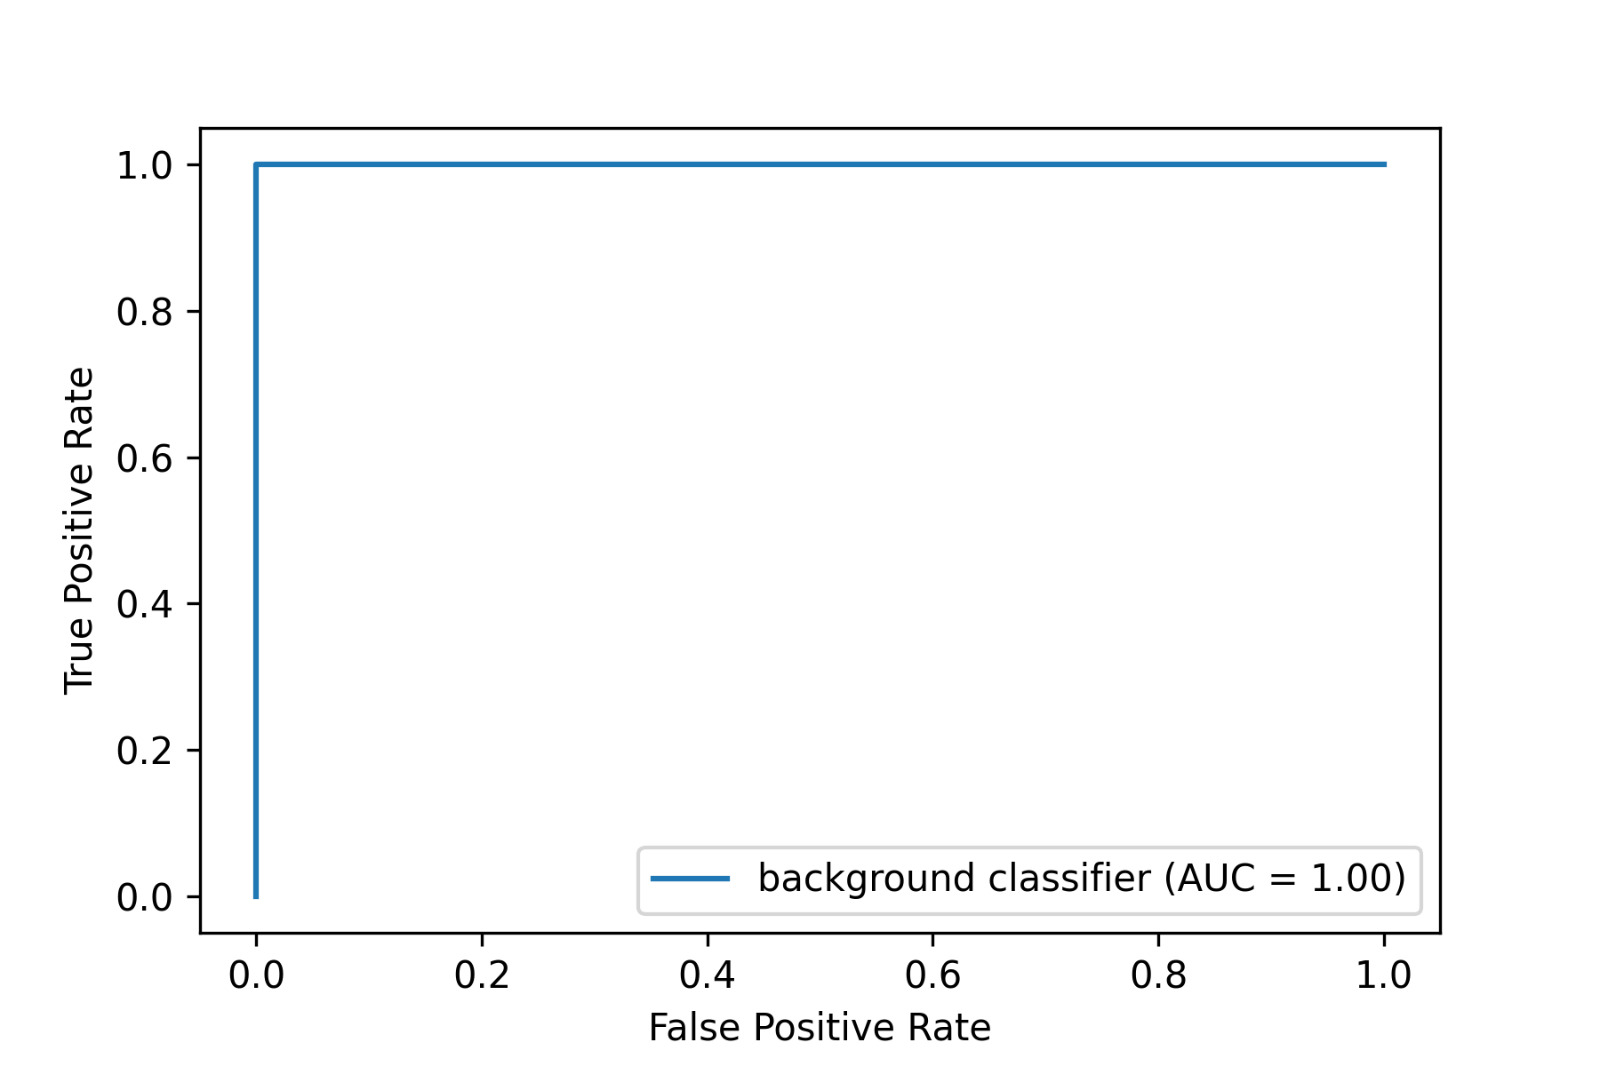
\includegraphics[scale=0.3]{img/background.png}
\caption{Curvas ROC para cada clase}\label{fig:roc}
\end{figure}

Profundizando en estos clasificadores de una única clase se determina 
\begin{table}[!]
  \centering
  \begin{tabular}{|c|c|c|c|}
    \hline
    Class & Precision & Recall & F1-Score \\
    \hline
    F & 0.81 & 0.87 & 0.84 \\ \hline
    T & 0.5 & 0.4 & 0.44 \\  
    \hline
  \end{tabular}
  \caption{Análisis de predicción de banana}\label{tab:banana}
\end{table}

La Tabla \ref{tab:banana} demuestra que no se puede confiar en las predicciones de este modelos ya que falla en la mayoría de los casos en los que el resutado real es positivo.

\begin{table}[!]
  \centering
  \begin{tabular}{|c|c|c|c|}
    \hline
    Class & Precision & Recall & F1-Score \\
    \hline
    F & 1 & 0.82 & 0.9 \\ \hline
    T & 0.82 & 1 & 0.9 \\  
    \hline
  \end{tabular}
  \caption{Análisis de predicción de wine}\label{tab:wine}
\end{table}


\begin{table}[!]
  \centering
  \begin{tabular}{|c|c|c|c|}
    \hline
    Class & Precision & Recall & F1-Score \\
    \hline
    F & 0.94 & 1.00 & 0.97 \\ \hline
    T & 1.00 & 0.75 & 0.86 \\  
    \hline
  \end{tabular}
  \caption{Análisis de predicción de background}\label{tab:background}
\end{table}

Sin embargo, la tabla \ref{tab:wine} y la tabla \ref{tab:background} permite ver que la precisión del modelo es muy fiable tanto si se produce el caso buscado como si no.


\section{Conclusión y Futuro Trabajo}
Mediante los resultados obtenidos en el apartado anteriror se concluye que los mejores atributos para un clasificador de las tres clases emplea como atributos clave la varianza, la diferencia entre los valores máximos y mínimos de cada sensor y le media de temperaturas y humedad que se producen a lo largo de todas las medidas tomadas durante cada una de las inducciones.  Para la predicción de una clase se considera que la mejor configuración de atributos es la variación de los valores que toman los sensores. La selección de estos atributos viene dada a que se pueden apreciar grandes modificaciones en los resultados cuando los sensores son sometidos a un estímulo, de esta forma, tiene sentido que la varianza y la diferencia entre sus valores máximos y mínimos sean buenos atributos para clasificar este conjunto de datos. Adicionalmente podemos determinar que los valores de la humedad y temperatura pueden ser a su vez relevantes ya que pueden afectar a la detección de valores de los distintos sensores. \\ \\
Para concluir, determinamos que los mejores modelos para predecir cualquier clase son los de Regresión  Logística y de XDB, mientras que para predecir una sola clase se recomienda utilizar el clasificador de Random Forest. Los valores de estos modelos son aceptables para todos los casos exceptuando la predicción única de la clase banana.\\

% ****************************************************************************
% BIBLIOGRAPHY AREA
% ****************************************************************************

\begin{thebibliography}{9}

\bibitem{Humidity}
Ramon Huerta, Thiago Mosqueiro, Jordi Fonollosa, Nikolai Rulkov, Irene Rodriguez-Lujan. 
\textit{Online Decorrelation of Humidity and Temperature in Chemical Sensors for Continuous Monitoring. Chemometrics and Intelligent Laboratory Systems 2016. }


\bibitem{Pandas}
Pandas. McKinney, W., and others. (2010). 
\textit{Data structures for statistical computing in python. In Proceedings of the 9th Python in Science Conference (Vol. 445, pp. 51–56).}

\bibitem{Numpy}
Numpy. \textit{Oliphant, T. E. (2006). A guide to NumPy (Vol. 1). Trelgol Publishing USA.}

\bibitem{Sci-kit}
Sci-kit Learn. \textit{Pedregosa, F., Varoquaux, Ga"el, Gramfort, A., Michel, V., Thirion, B., Grisel, O., … others. (2011). Scikit-learn: Machine learning in Python. Journal of Machine Learning Research, 12(Oct), 2825–2830.}

\bibitem{Matplotlib}
Matplotlib. \textit{Hunter, J. D. (2007). Matplotlib: A 2D graphics environment. Computing in Science amp; Engineering, 9(3), 90–95.}

\bibitem{LazyPredict}
LazyPredict. \\\texttt{https://github.com/shankarpandala/lazypredict}

\bibitem{keras}
Keras. \textit{Chollet, F.,  others. (2015). Keras. GitHub. Retrieved from} \\\texttt{https://github.com/fchollet/keras}

\bibitem{XGBoost}
XGBoost. \textit{Tianqi Chen and Carlos Guestrin. XGBoost: A Scalable Tree Boosting System. In 22nd SIGKDD Conference on Knowledge Discovery and Data Mining, 2016}

\bibitem{LightGBM} 
LightGBM.  \textit{Guolin Ke, Qi Meng, Thomas Finley, Taifeng Wang, Wei Chen, Weidong Ma, Qiwei Ye, Tie-Yan Liu. "LightGBM: A Highly Efficient Gradient Boosting Decision Tree". Advances in Neural Information Processing Systems 30 (NIPS 2017), pp. 3149-3157.}

\end{thebibliography}



% ****************************************************************************
% END OF BIBLIOGRAPHY AREA
% ****************************************************************************

\end{document}
